\begin{abstract}
    Multidimensional categorical data is widespread but not easily visualized using standard methods. For example, questionnaire (e.g. survey) data generally consists of questions with categorical responses (e.g., yes/no, hate/dislike/neutral/like/love). Thus, a questionnaire with 10 questions, each with five mutually exclusive responses, gives a dataset of $5^{10}$ possible observations, an amount of data that would be hard to reasonably collect. Hence, this type of dataset is necessarily sparse. Popular methods of handling categorical data include one-hot encoding (which exacerbates the dimensionality problem) and enumeration, which applies an unwarranted and potentially misleading notional order to the data. To address this, we introduce a novel visualization method named Data Reduction Network (DRN). Using a network-graph structure, the DRN denotes each categorical feature as a node with interrelationships between nodes denoted by weighted edges. The graph is statistically reduced to reveal the strongest or weakest path-wise relationships between features and to reduce visual clutter. A key advantage is that it does not “lose” features, but rather represents interrelationships across the entire categorical feature set without eliminating weaker relationships or features. Indeed, the graph representation can be inverted so that instead of visualizing the strongest interrelationships, the weakest can be surfaced. The DRN is a powerful visualization tool for multi-dimensional categorical data and in particular data derived from surveys and questionaires.
\end{abstract}

\subsection{Introduction}\label{introduction}

The proliferation of Big Data has opened new frontiers in the analysis of information across numerous disciplines. This surge of data is most pronounced in areas such as large-scale surveys, which provide a wealth of multidimensional data capable of answering diverse research questions that may not be easily tested in experimental lab settings \citep{Manyika2011BigDT}. However, the size and complexity of this type of data introduce unique challenges, particularly in the domain of data visualization and downstream analysis.

For example, questionnaire (e.g., survey) data are generally categorical with just a few alternatives for each question, as with the Likert scale that typically consists of five alternatives for each question (e.g., \texttt{strongly agree}, \texttt{agree}, \texttt{neutral}, \texttt{disagree}, \texttt{strongly disagree}). Consider a small survey with ten questions, each with five alternatives, which produces $5^{10} (9,765,625)$ possible distinct completed questionnaires. In practice, visualizing such a large amount of data in an elegant format is rarely feasible. Rather, the standard approach is to consider a few questions and marginalize (i.e., sum) over the remaining responses. A summary headline result could be that ``90\% of respondents strongly agree with Question 1''. Another could be ``75\% of respondents strongly agree with Question 2'' and so on. However, this approach does not provide information on the respondents who selected \texttt{strongly agree} for both Questions 1 and 2. Even more troubling, there could be a third question that is strongly related to both questions but has been marginalized over, potentially leading to issues like Simpson's paradox \citep{hernan2011simpsons}, a phenomenon where a trend or relationship that appears within different groups reverses or disappears when the groups are combined, thus misleading the overall analysis.

As with our survey example above, categorical data often exists in a high-dimensional space. The challenge lies in accurately representing multiple dimensions on a two or three-dimensional plane, which carries potential risks, from oversimplification to cognitive overload \citep{fayyad2002information}. This complexity is amplified by the heterogeneous nature of survey data, which may comprise multiple choice and open-ended responses to Likert scales, each necessitating different visualization techniques \citep{shneiderman1996eyes}. Current common methods to generate informative visualizations for high dimensional categorical data include manually pre-selecting questions or dimensional reduction techniques such as principal component analysis (PCA) and t-distributed stochastic neighbor embedding \citep{Wong1997MultivariateVU}. These techniques may help to inform some conclusions, yet they may still not be fully comprehensible to non-expert audiences or require excessive human effort to filter the information. In the filtering process, some important relationships, such as joint respondents between two questions, may be omitted due to data oversimplification. Furthermore, such oversimplification may even lead to bias in the downstream analysis.

One popular method for addressing high-dimensional categorical data is through one-hot encoding. In this method, each level of the data element is mapped into a string of $n$-bits where $1$ marks the specific response for that row. For example, using the Likert scale, one-hot encoding produces a string of five bits where \texttt{10000} corresponds to \texttt{strongly agree} for that particular response and \texttt{01000} for the \texttt{agree} response. Suppose you have a data frame with rows corresponding to survey respondents and columns corresponding to questions. For each question, one-hot encoding will generate five bits. As a result, for $n$ original columns, there will now be $5n$ one-hot encoded columns. Although it is relatively simple to see this two-dimensional data as a binary array, the relationships between the respondents (rows) and the survey questions (columns) may not be apparent from this representation.

Another common technique is label-encoding where each categorical level is mapped to an integer. For example, if our category is \texttt{favorite fruit} with levels \texttt{apple}, \texttt{banana}, and \texttt{strawberry}, then with label encoding, we have \texttt{apple} $\rightarrow 1$, \texttt{banana} $\rightarrow 2$, and \texttt{strawberry} $\rightarrow 3$. The problem with this approach lies in the inherent ordering of integers, which may not reflect the true nature of the categories. For example, because $2 > 1$, does that imply that \texttt{banana} is somehow more than \texttt{apple}? The downstream numerical analysis relies on numeric properties and is oblivious to the nuances expressed by the categorical variable. This lack of sensitivity can lead to spurious correlations or nonsensical results.

To distill insightful and actionable visualizations from large survey data, it is essential to balance the trade-off between simplicity and completeness, highlighting the most critical variables for downstream data processing \citep{wardlow2022perceptions}. One previous attempt involves using the cobweb diagram to represent the inter-relationships between nodes \citep{upton2000cobweb}. This method effectively distills the complexity in high dimensional contingency tables, but may not be easily comprehensible to those without expertise. In this paper, we propose the Data Reduction Network (DRN) method, a straightforward visualization for representing multidimensional categorical data. The DRN method generates a condensed network graph, emphasizing the strong interrelationships among the variables. By employing a maximum spanning tree, the network not only avoids the risk of oversimplification but also retains the most significant insights from the survey.

\subsection{Method}\label{Method}
% The actual structure of DRN (i.e. how is it constructed)

\begin{table}
    \begin{tabular}[c]{||c c c c c||}
        \hline
        \textbf{Unit} & \textbf{Question 1} & \textbf{Question 2} & \ldots & \textbf{Question N} \\
        \hline\hline
        1 & yes & sometimes & \ldots & responseN \\
        2 & no & never & \ldots & responseK \\
        3 & yes & never & \ldots & responseN \\
        \ldots & \ldots & \ldots & \ldots & \ldots \\
        \hline
    \end{tabular}
    \caption{Sample Survey Data Table. Each row represents a participant's response record and each column corresponds to questions in the survey.}
    \label{tab:table1}
\end{table}

\begin{table}
    \begin{tabular}[c]{||c c c c c||}
        \hline
        \textbf{Unit} & \textbf{Question 1} & \textbf{Question 2} & \ldots & \textbf{Question N} \\
        \hline\hline
        1 & 1 & 3 & \ldots & 6 \\
        2 & 2 & 4 & \ldots & 2 \\
        3 & 1 & 4 & \ldots & 6 \\
        \ldots & \ldots & \ldots & \ldots & \ldots \\
        \hline
    \end{tabular}
    \caption{Survey data table where each response is converted to an integer number.}
    \label{tab:table2}
\end{table}

\begin{table}
    \begin{tabular}[c]{||c c c c c||}
        \hline
        \textbf{Unit} & \textbf{Question 1} & \textbf{Question 2} & \ldots & \textbf{Question N} \\
        \hline\hline
        1 & Q1-1 & Q2-3 & \ldots & QN-6 \\
        2 & Q1-2 & Q2-4 & \ldots & QN-2 \\
        3 & Q1-1 & Q2-4 & \ldots & QN-6 \\
        \ldots & \ldots & \ldots & \ldots & \ldots \\
        \hline
    \end{tabular}
    \caption{Survey table with labeled response and corresponding questions.}
    \label{tab:table3}
\end{table}

\begin{table}
    \begin{tabular}[c]{||c c c c||}
        \hline
        \textbf{Unit} & \textbf{Question 1} & \textbf{Question 2} & \textbf{Question 3} \\
        \hline\hline
        1 & Q1-1 & Q2-3 & Q3-6 \\
        2 & Q1-1 & Q2-4 & Q3-6 \\
        3 & Q1-2 & Q2-4 & Q3-2 \\
        \hline
    \end{tabular}
    \caption{Survey table with further transformed responses label. Now each label will have the question number in them.}
    \label{tab:table4}
\end{table}

\begin{figure}[]
    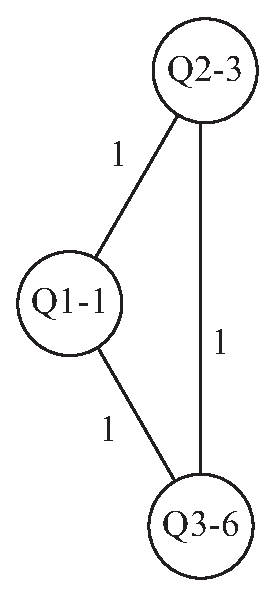
\includegraphics[height=15em]{clique.eps}
    \caption{A clique representation of the first respondent in the hypothetical example.}
    \label{clique}
\end{figure}

\begin{figure}[]
    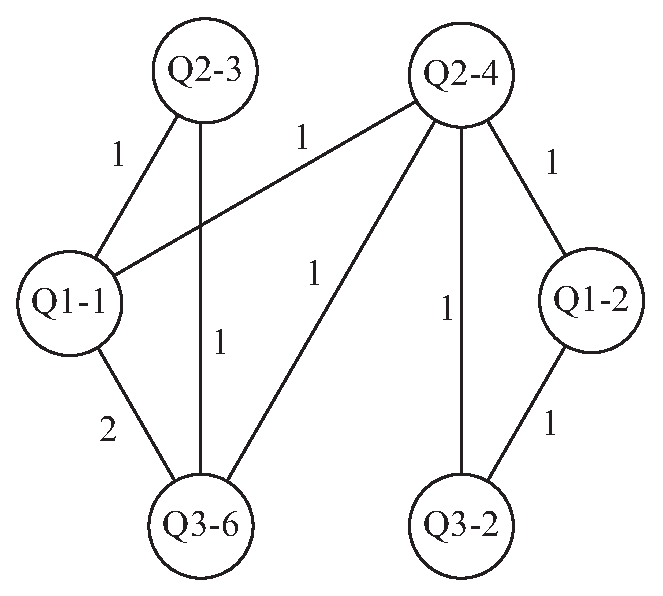
\includegraphics[height=15em]{graph.eps}
    \caption{Network illustrating responses from the first 3 rows of the response table.}
    \label{graph}
\end{figure}

\begin{figure}[]
    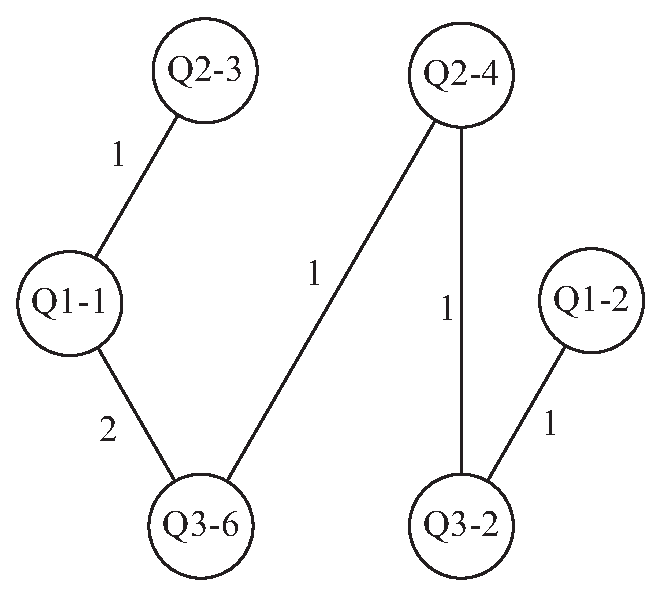
\includegraphics[height=15em]{tree.eps}
    \caption{Network after maximum spanning tree.}
    \label{tree}
\end{figure}

The DRN is a graph composed of nodes and edges. Each node denotes the answer to a particular survey question, whereas the edges between nodes indicate the co-occurrence of respective answers.  The DRN maintains a running tally of the number of times an edge occurs in the dataset, as well as the frequency of a particular response to a given question.

Suppose we have a set of survey data shown in \autoref{tab:table1}. For the sake of convenience and visual simplicity, we map each response to an integer (e.g., yes $\to$ 1, no $\to$ 2, sometimes $\rightarrow 3$) as demonstrated in \autoref{tab:table2}. It is worth noting that while this is technically a label encoding process, it is an optional process. The node \texttt{Q1\_1} could have been labeled \texttt{Q1\_yes} but it is clear that visual clutter would soon ensue for more complex responses like \texttt{Q3\_responseK}. By employing this encoding technique, we achieve a concise representation of each question-response pair, as demonstrated in \autoref{tab:table3}. This gives every entry in the table a code that indicates the question-response pair. Each row in the table corresponds to a respondent. It is possible for two respondents to answer the survey in exactly the same way, leading to duplicated rows in the table.

Once the data is properly encoded, the subsequent step is to construct the DRN where each entry from the table represents a node, and the edges symbolize the connections between these nodes. This means that each row generates a \textit{clique}, a network of mutually connected nodes, and these cliques are merged to create a comprehensive clique whose edges count all joint responses for the entire table.

The process of constructing a master graph from the table is a two step process:
\begin{enumerate}
    % \renewcommand{\labelenumi}{(\roman{enumi})}
    \item Form a clique for every row
    \item Merge the cliques by accumulating the edge counts
\end{enumerate}
\noindent Following a hypothetical example with three questions shown in \autoref{tab:table4}, we start with the first row, each question-response term becomes a node and there is an edge between every two terms in this row with weight $1$. The clique formed from the first row is depicted in \autoref{clique}. After completing cliques for all rows, three in this case, they are merged into a master graph where the edge counts are accumulated as shown in \autoref{graph}. Please note that in this case, the edge between \texttt{Q1\_1} and \texttt{Q3\_6} occurs in two of the cliques so it is weighted $2$.

For large datasets, these master graphs can become extremely dense and impossible to interpret. To simplify the graph and reveal the key statistically significant relationships, we employ \texttt{networkx}'s \texttt{maximum\_spanning\_tree} function, which applies Prim's algorithm \citep{dijkstra1959note}. This algorithm calculates the maximum spanning tree where the weights are the edge counts. It's worth mentioning that Prim's algorithm is a greedy algorithm that finds a maximum spanning tree for a weighted undirected graph. Furthermore, it's worth noting that any maximum spanning tree algorithm could be used. For instance, Kruskal's algorithm \citep{kruskal1956shortest}, also supported by \texttt{networkx} \citep{SciPyProceedings_11}, is a valid alternative.

The resulting tree maintains the largest edge-weights, which are the strongest co-occurring responses. It is worth noting that the maximum spanning tree might not be unique; hence, in the event of a tie, any competing tree could be chosen. With large combinatorial complexity associated with large data sets such ties are unlikely. In the present example, one maximum-spanning tree is shown in \autoref{tree}

Given that the edges in the DRN represent the tallies of co-occurring survey responses, these values align with those found in a contingency table that encompasses the variables represented by the nodes. Therefore, the DRN effectively $unrolls$ a high-dimensional contingency table onto a network graph, thereby facilitating the identification of the strongest inter-relationships. DRNs facilitate inferential statistics by translating topological features, such as clusters and connections in the graph, into statistical quantities of interest.

\subsection{Example}\label{Example}
\subsubsection{The Solar Flare Dataset}
% Dataset Description


\begin{table*}
    \begin{tabular}{l|l}
        \hline
        \textbf{Feature} & \textbf{Description} \\
        \hline
        klass & Code for class (modified Zurich class) (A, B, C, D, E, F, H) \\
        size & Code for largest spot size (X, R, S, A, H, K) \\
        dist & Code for spot distribution (X, O, I, C) \\
        act & Activity (1 = reduced, 2 = unchanged) \\
        evo & Evolution (1 = decay, 2 = no growth, 3 = growth) \\
        prev & Previous 24 hour flare activity code (1 = nothing as big as an M1,2 = one M1,3 = more activity than one M1) \\
        complex & Historically-complex (1 = Yes, 2 = No) \\
        hist\_complex & Did region become historically complex on this pass across the sun's disk (1 = yes, 2 = no) \\
        area & Area (1 = small, 2 = large) \\
        c\_class & Small with few noticeable consequences on Earth \\
        m\_class & Medium-sized; cause brief radio blackouts that affect Earth's polar regions \\
        x\_class & Big; major events that can trigger planet-wide radio blackouts and long-lasting radiation storms \\
        \hline
    \end{tabular}
    \caption{Table for the features described in the solar flare dataset.}
    \label{data_features}
\end{table*}

\begin{figure}[]
    \noindent
    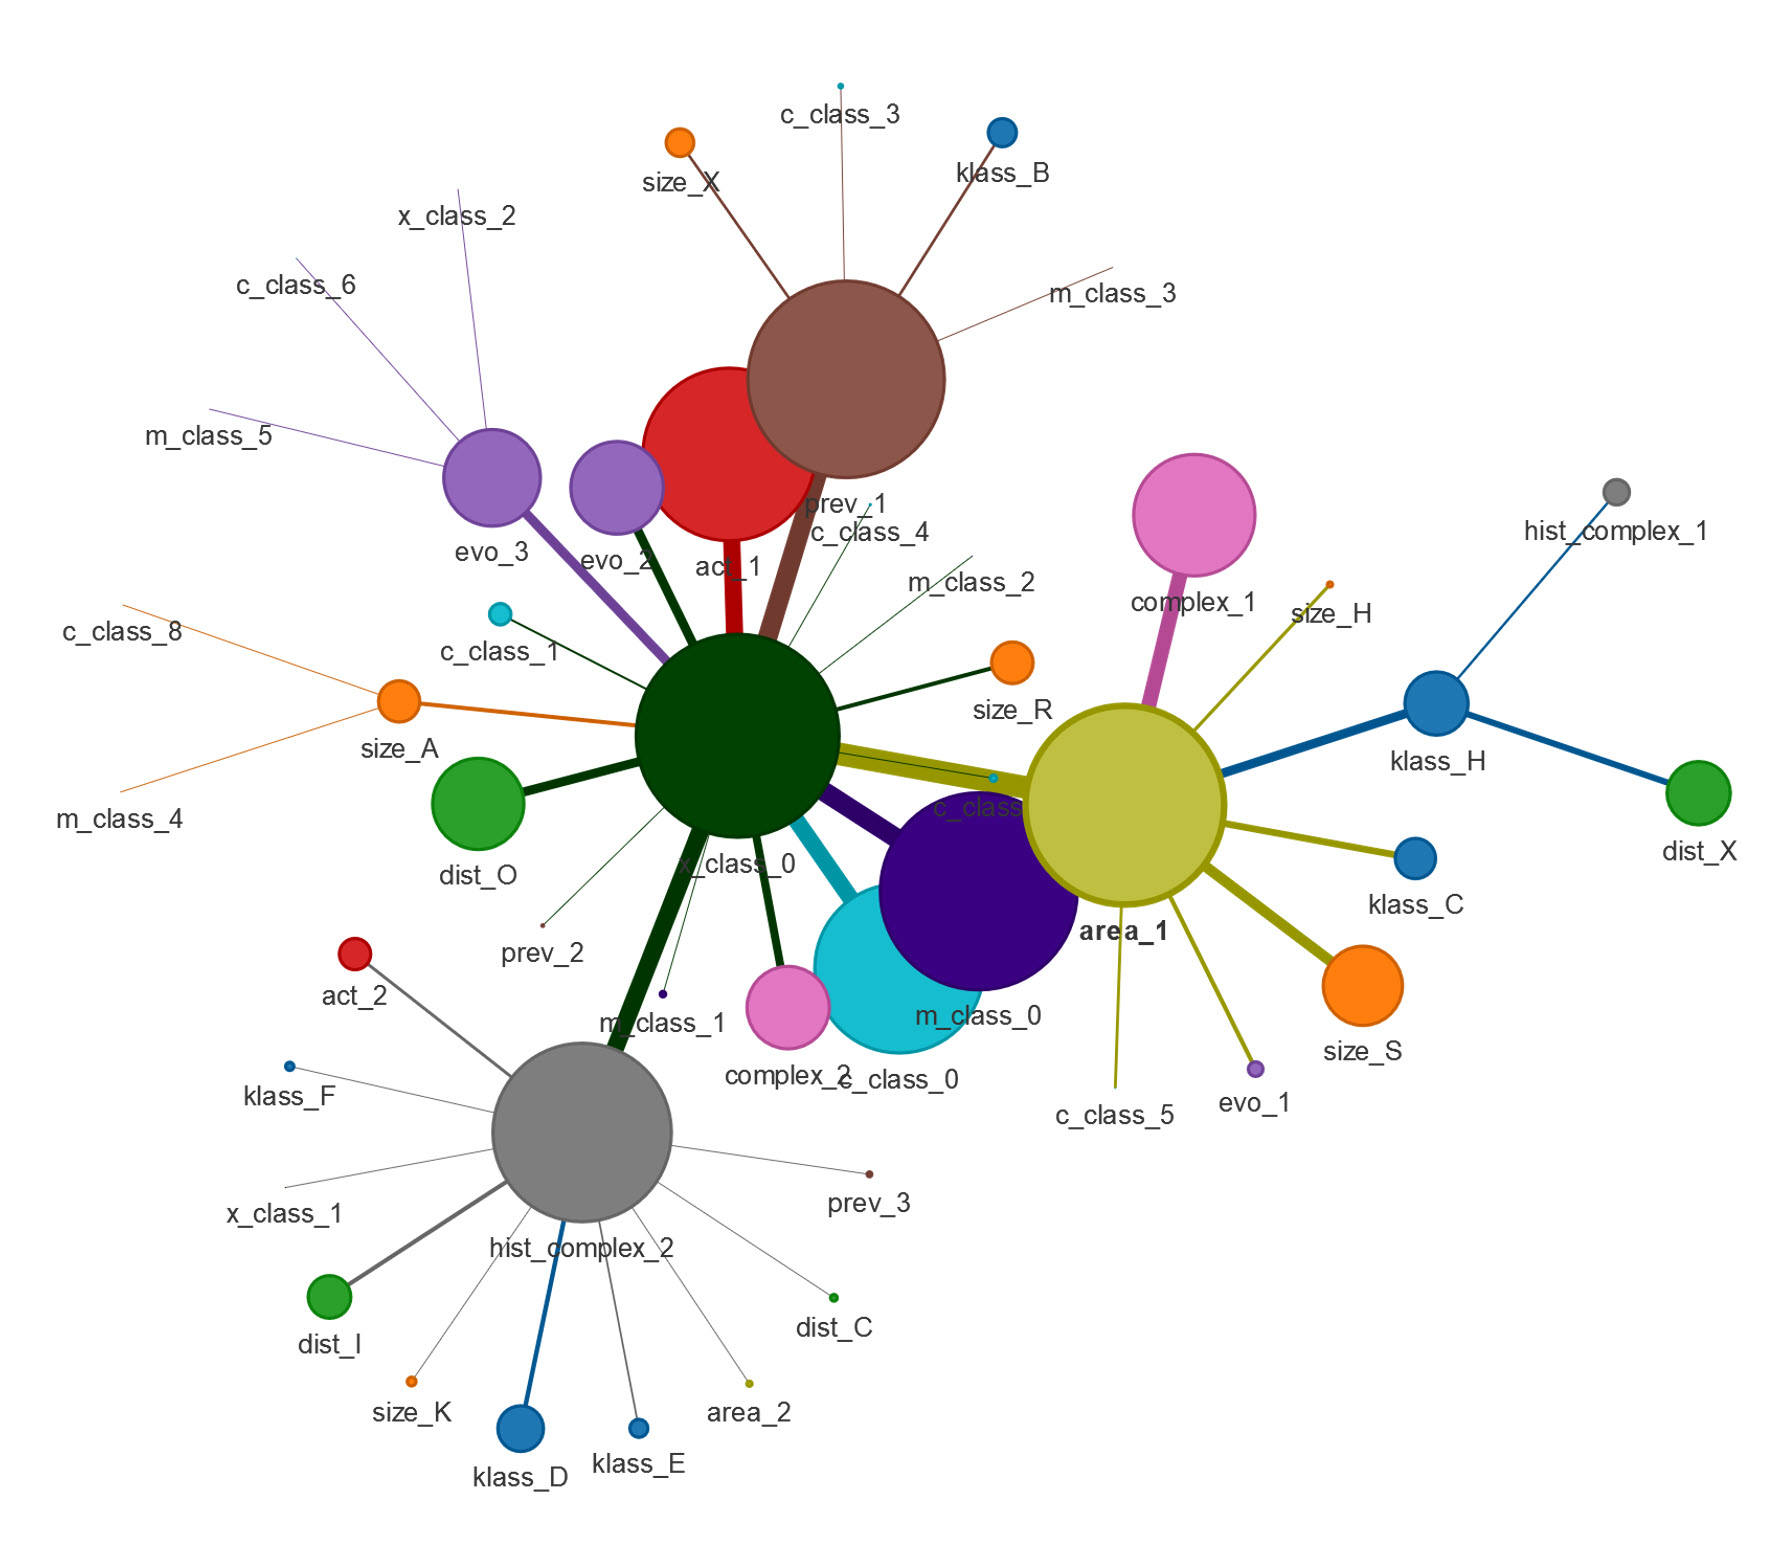
\includegraphics[width=\columnwidth]{solar_flares.jpg}
    \caption{An overview of DRN for the solar flare dataset}
    \label{solar}
\end{figure}

As an example, a simple dataset is presented. The Solar Flare Dataset was adopted from University of California at Irvine (UCI) Machine Learning Repository\footnote{http://archive.ics.uci.edu/ml/datasets/solar+flare}. Each entry of the dataset describes multiple features of an active region on the sun as well as the number of flares events that occurred within the past 24 hours in the region. The features were described in \autoref{data_features}.  We've also provided this in an example Jupyter notebook, the link to which can be found in the conclusion section of this document.

\autoref{solar} shows the DRN representation of the Solar Flare Dataset. In addition to the methods mentioned in the previous section, for clarity edge weights are not explicitly shown but translated into edge thickness with the most common occurrence of responses having heavier lines. Additionally, the size of the nodes is proportional to the number of responses for the particular question-response. Finally for added clarity, the responses associated with each question are encoded with the same color making it easy to discern which responses belong to which question. Each feature is encoded as a single label. For example, for the feature \texttt{act}, there are two options: 1 (reduced), and 2 (unchanged). If a region has reduced solar activity, the feature will be encoded as \texttt{act\_1}. This code will appear in the DRN as nodes and the size of the node is proportional to the number of entries that contains the corresponding feature coding. In other words, greater node size indicates the most prevalent features across all entries.

In \autoref{solar}, the largest node in the center was \texttt{x\_class\_0}, which indicates that for most active regions on the sun, 0 x-class solar flare activity was observed. While it shows the specific feature encoding for that feature category, the DRN could also reveal joint encoding relationships through the edge connection and the thickness of edges. Thicker edges indicate stronger correlations between two features. For example, regions that have the feature label of \texttt{x\_class\_0} will also most likely have the features of \texttt{area\_1}, \texttt{act\_1}, \texttt{m\_class\_0}, \texttt{prev\_1}, \texttt{hist\_complex\_2}, \texttt{c\_class\_0}, \texttt{evo\_3}, as indicated by the thickness of the edge. This indicates that regions that do not have x-class solar flare activity, they would most likely be 1) small area, or 2) regions with reduced activity, or 3) no m-class solar flare activity, or 4) not as big as M1, or 5) wasn't considered as historically complex, or 6) no c-class solar flare activity, or 7) actively growing. Notice that each edge represents an independent joint relationship with each other.

\subsection{Use Case\label{Use Case}}
\subsubsection{Telehealth Questionnaire\label{Telehealth}}
\begin{table*}
    \begin{tabular}[c]{p{0.07\DUtablewidth}p{0.09\DUtablewidth}p{0.6\DUtablewidth}p{0.25\DUtablewidth}}
        \toprule
        \textbf{Label} & \textbf{Annotation} & \textbf{Response description} & \textbf{Respondent's Response}  \\
        \midrule
        Q11-2 & A & People over a certain age cannot be well cared for using telehealth & \textbf{TRUE} \\
        Q11-3 & B & The older adults I serve do not always have access to the resources needed to make a telehealth visit effective & \textbf{TRUE} \\
        Q11-5 & C & I have concerns about the impact of telehealth on fragmentation of care for older adults & \textbf{TRUE} \\
        Q11-6 & D & Relationship building via telehealth is more difficult than in person & \textbf{TRUE} \\
        Q11-7 & Ba & There is a lack of support from my health system leadership or support staff to make telehealth for my older adults an effective alternative & \textbf{TRUE} \\
        Q11-8 & Bb & Providing telehealth is dangerous to older adults because their care needs are so medically complex & \textbf{TRUE} \\
        \bottomrule
    \end{tabular}
    \caption{Table for response description and annotation used in \autoref{Overview}.}
    \label{tab:telehealth1}
\end{table*}


\begin{table*}
    \begin{tabular}[c]{p{0.07\DUtablewidth}p{0.09\DUtablewidth}p{0.6\DUtablewidth}p{0.25\DUtablewidth}}
        \toprule
        \textbf{Label} & \textbf{Annotation} & \textbf{Response description} & \textbf{Respondent's Response}  \\
        \midrule
        Q11-4&Da&(Subquestion 4) Older adults’ significant physical or cognitive challenges make telehealth unrealistic&\textbf{TRUE}\\
        Q2&Db&For demographic purposes only, select all that describe your ethnic background?&\textbf{White/Caucasian}\\
        Q9&Dc&Which of the following best describes the top THREE reasons that you feel some older adults may not use telehealth? Please choose THREE:&\textbf{Older adults’ physical and/or cognitive challenges}\\
        \bottomrule
    \end{tabular}
    \caption{Response description for DRN in \autoref{DTree2}}
    \label{tab:telehealth2}
\end{table*}

In this section, we demonstrate an application of the DRN, using it to analyze a complex survey dataset. This dataset was obtained from a survey of the perceptions and uses of telehealth in the care of older adults \citep{wardlow2022perceptions}. The survey used a questionnaire with 29 close-ended questions, spanning multiple-choice, agreement scale, dichotomous true/false, and rating scale formats. These statements presented potential challenges associated with using telehealth to serve older adults, touching on areas like relationship building, high medical complexity, physical and cognitive impairment, and fragmentation of care. The survey captured responses from 7246 U.S. clinicians across a range of specialties.\footnote{The exact questionnaire can be found at:\ \url{https://pubmed.ncbi.nlm.nih.gov/36493377/}}

\autoref{Overview} depicts an overview of the DRN for the entire survey. We've followed a specific convention for labeling each node. When questions include subquestions, the corresponding response is represented with a hyphenated label connecting the question number, subquestion number, and numeric representation of the response. For instance, a \textbf{TRUE} response for question 11 subquestion 4 is labeled as \texttt{Q11-4\_90}. The numeric representation of the response can be arbitrary but to avoid confusion the coding used in the survey results itself was used where  \textbf{TRUE} is represented as $90$. For questions without subquestions, we simply omit the hyphen and subquestion number, e.g., \texttt{Q2\_91}.

Each node's size is proportionate to the number of respondents who chose the associated answer, with larger nodes representing the most common question-answer combinations (topline results). For ease of discussion, the most prominent nodes in \autoref{Overview} are labeled with uppercase letters, and two other nodes of interest with an uppercase-lowercase pair. \autoref{tab:telehealth1} complements the figure by detailing the annotation, DRN label, and corresponding question-answer pairs for these nodes.

The prominent nodes, labeled as A, B, Ba, Bb, C, and D in the network diagram, are derived from the subquestions of survey Question 11. This question presented a list of reasons why providers might choose to exclude older adults from their telehealth services, and asked respondents to rate their agreement with each statement, based on their personal and professional opinions. The full text of Question 11 is as follows:

\begin{quotation}
\noindent Q11: The following is the list of reasons why some providers might choose to exclude older adults from their telehealth offerings (visits, program, system). Please read and indicate your personal and professional opinion about whether you believe each statement is true or false
\end{quotation}

The prominent nodes indicate the most frequently selected responses across all survey participants. Observations from these responses allow for immediate conclusions to be drawn across all U.S. clinical specialties. The most common reasons to exclude telehealth offerings for older patients include: 1) the belief that telehealth couldn't provide sufficient healthcare service to older patients, 2) concerns about whether older patients have enough resources to properly utilize the service, and 3) possible insufficiency of resources by the medical staff to offer the telehealth service. These conclusions serve as the top-line information extracted from the questionnaires.

Similar to the DRN analysis of the solar flare dataset, the strength of joint responses among all respondents is visually emphasized by the width of the lines (i.e., edges) connecting the nodes. Employing the maximum spanning tree method, the DRN selectively showcases the most significant joint relationships within the network. To illustrate, a thicker edge connecting nodes A and B indicates that respondents who selected response B also likely selected response A. In terms of raw data, the count of respondents who selected both responses A and B is notably higher than any other pairwise combination. In sum, the DRN not only indicates topline responses but also captures significant joint responses.

The tree-like structure of the DRN further allows the isolation of individual trees within the network, thus providing supplementary visual information for a particular response. For example, \autoref{DTree2} shows a detailed view of the tree segment centered around node D for closer examination.  For clarity, the most prominent nodes within this tree are annotated according to \autoref{tab:telehealth2}.

This tree allows us to see the interconnections between various survey responses. Notably, respondents who agreed that "relationship building via telehealth is more difficult than in person" (D), also agreed with the statements "older adults’ significant physical or cognitive challenges make telehealth unrealistic" (Da) and "older adults’ physical and/or cognitive challenges is one of the reasons why older patients may refuse to use telehealth" (Dc).

In addition, most respondents who agreed with the difficulties of relationship building via telehealth identified as White/Caucasian (Db). However, this trend might be reflective of the ethnic imbalance in our respondents.

Additionally, upon closer inspection of the Da node, we see that most respondents who expressed concerns about cognitive/physical decline disagreed with the statement "insufficient resources to effectively use telehealth service" (denoted by the light green node Q11-3\_26 under Da).

A quick glance at the network offers substantial insights. It becomes clear that the majority of respondents in this survey shared opinions on the potential reasons why providers might exclude older adults from telehealth services (Q11). They largely agreed on three primary factors that make telehealth less suitable for people over a certain age: 1) difficulties in relationship building, 2) potential fragmentation of care, and 3) a lack of resources. Those who indicated a lack of resources as a potential issue further specified that there is a lack of support from the health system leadership or support staff to make telehealth effective. For respondents who indicated the difficulties of relationship building would be a potential issue, the majority of them further specify that older adults’ significant physical or cognitive challenges would make telehealth unrealistic.

The majority of the participants expressing concerns about elder physical or cognitive challenges disagreed with the insufficient resource argument. It is also noteworthy that most participants who identified difficulties in relationship building as a major concern reported their ethnic background as white/Caucasian.

This example demonstrates how the DRN offers a clean, concise visualization that enables users to quickly identify relationships between different questions in a survey. It not only highlights the topline information but also allows users to explore additional relevant data associated with each topline piece of information through the examination of the edges. Compared to traditional methods, DRN provides a simpler, yet more informative, visualization of survey data.



\begin{figure*}[]
    \noindent
    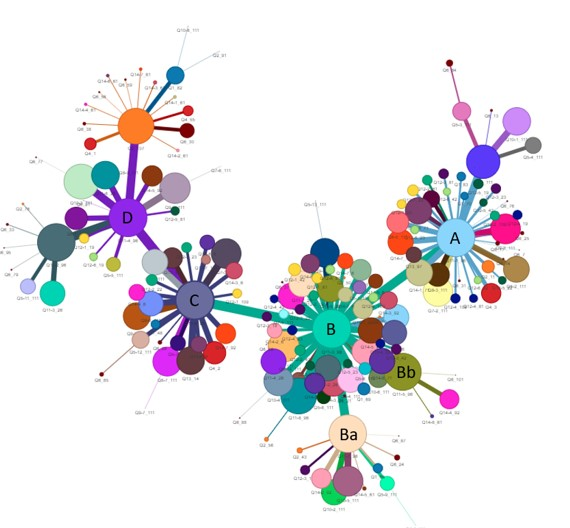
\includegraphics[width=\textwidth]{Overview-v3.jpg}
    \caption{An overview of DRN for the telehealth questionnaire \label{Overview}}
\end{figure*}

\begin{figure}[]
    \noindent
    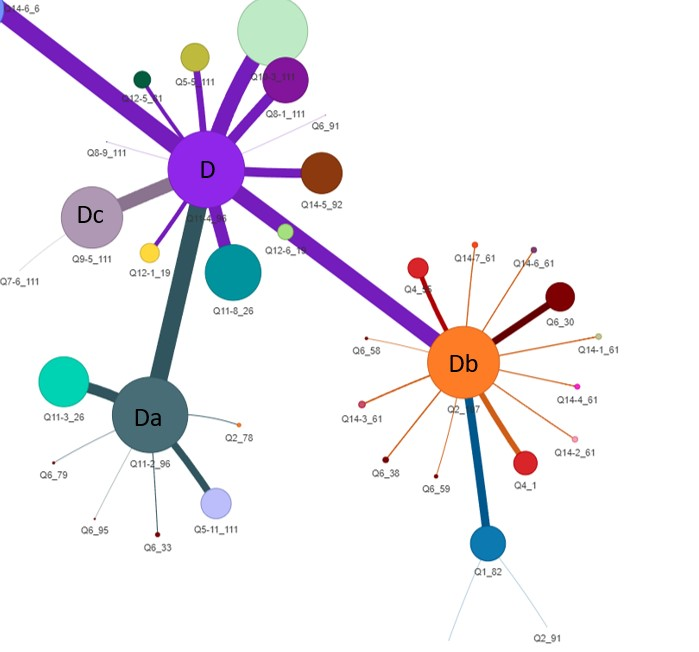
\includegraphics[width=\columnwidth]{Tree-D.jpg}
    \caption{A closer look at tree D from the telehealth questionnaire\label{DTree2}}
\end{figure}

\subsection{Discussion} \label{Discussion}

Data Reduction Networks (DRNs) provide a valuable solution in the field of data exploration tools, predominantly addressing the handling of categorical data, which has often been overlooked by tools focusing on continuous data. As previously noted, the DRN is adept at rapidly highlighting top-line information. It effectively highlights significant relationships, which can be challenging to discern when dealing with high-dimensional contingency tables. While contingency tables are useful for data analysis, they can become intractable beyond a few dimensions and may be too cumbersome for data exploration.

Despite their utility, DRNs share the same limitations common to data exploration tools. Specifically, a DRN's purpose isn't to act as a standalone data analysis tool, even though it can highlight interesting aspects of a data set. Instead, its strength lies in fostering hypotheses that prompt further investigation, either within the existing data set or via the acquisition of new, targeted data.

The utility of DRNs is not confined to survey data. In fact, categorical data can be seen as analogous to survey data, where features map to questions, and feature values correspond to answers. The example of solar flares showcases this equivalence. Although largely a semantic shift, it reframes the data's context. By contrast, our telehealth use case involves the use of actual survey data.

In the presence of continuous data in data sets, discretization or binning techniques akin to those utilized in decision trees can be employed to convert this data into a categorical form. However, this conversion introduces a new challenge - bin formulation. Still, this can be tackled by using existing techniques from decision tree methodologies \citep{garcia}.

A unique problem with survey data comes from questions where multiple responses are permitted. Even visualization methods that can accommodate categorical data struggle with this. The DRN elegantly handles this by generating cliques based on all responses from a respondent, irrespective of whether those responses are associated with different or the same question.

Regarding data imbalances, especially those of a demographic nature, traditional methods such as oversampling underrepresented populations may inadvertently amplify certain relationships in the DRN. As an alternative, removing the overrepresented node and its edges from the main graph, creating a new tree devoid of this node. This action can result in a graphical representation where the influence of the overrepresented node is neutralized, but relationships that may involve that overrepresented demographic are retained. This approach preserves the same weighting of the relationships without emphasizing the relationship to the overrepresented node. It falls on the analyst to weigh the merits of this approach versus the traditional oversampling techniques to determine which approach best fits their problem.

The extraction of a maximum spanning tree from the master graph within a DRN serves to capture prominent features in the survey data. However, this method may inadvertently overlook relationships that, while strong, are not the most dominant, and it would miss subtler, hidden insights. As a potential future direction, the application of alternative subgraph extraction or graph partitioning methods to the master graph might address this concern.

For further enhancement of its utility and streamlining of data exploration, several features could be incorporated into a DRN's graphical interface. An advanced user interface could enable the omission or disabling of nodes upon a user's request, and subsequently generate new trees accordingly. This would enable users to remove nodes based on their relevance or preference.  Another feature could enable a user to select a node, which would then prompt the UI to trigger a statistical function - for instance, constructing a contingency table based on the question associated with the selected node, and questions associated with all connected nodes. This feature could facilitate and streamline subsequent statistical analyses.

Considering the computational demands associated with processing large survey data, strategies such as parallel processing or employing graphics processing unit (GPU)-enhanced graph packages, like cugraph \citep{cugraph}, could significantly enhance processing efficiency.

DRNs offer a powerful tool for exploring categorical data, especially in survey data sets. While they have certain limitations, they excel at revealing important relationships and fostering hypotheses for further investigation. The adaptability of DRNs to various data types, including the treatment of continuous data and handling of multiple responses, contributes to their effectiveness. Future improvements to DRN's graphical interface could further enhance their utility, while alternative methods for extracting subgraphs could reveal subtler insights that might be missed by the current approach. Further studies are needed to explore these areas and continue refining the DRN methodology.

DRNs serve as potent tools for categorical data exploration, excelling at revealing key relationships and fostering investigatory hypotheses. Their versatility to handle various data types and responses boosts their efficacy. Future enhancements to the DRN methodology could offer deeper insights, but further research and development is needed.

\subsection{Conclusion} \label{Conclusion}

DRNs offer significant potential in the exploration of categorical data, as they can reveal crucial relationships and foster the generation of hypotheses for subsequent investigations. Their utility in data analysis is promising due to their flexible approach in accommodating diverse data types and responses. They are particularly effective in survey data analysis, where their unique ability to manage categorical data, including continuous data and multiple responses, is most apparent.

However, DRNs are not without their challenges. There is potential for future improvements to enhance their functionality and unlock more profound insights. Potential areas for improvement include the provision of a fully featured graphical interface, the development of alternative methods for subgraph extraction, and more sophisticated management of data imbalances and computational demands. Furthermore, more studies are needed to fully explore and refine the DRN methodology, ensuring that this powerful tool continues to evolve and contribute to the field of data exploration.

An example Jupyter notebook is available at our GitHub repository: \url{https://github.com/Westhealth/drn-scipy2023/}. The efforts to build the method to a library is documented in the \href{https://github.com/WestHealth/drn-scipy2023/blob/master/README.md}{\texttt{README}} file.

